% --------
% Preamble
% --------
\documentclass[12pt,a4paper]{article}

% Packages
\usepackage[utf8]{inputenc}
\usepackage[T1]{fontenc} % Font
\usepackage[spanish,es-tabla]{babel} % Idioma y tabla
\usepackage{gensymb} % Degree symbol
\usepackage{booktabs} % Custom tables
\usepackage{cite} % Bibliographie
\usepackage{fancyhdr} % Header and footnote
\usepackage{graphicx} % Floating figures
\usepackage{amsmath} % Advanced math
\usepackage{hyperref}
\usepackage{caption}
\usepackage{amsfonts}
\usepackage{amssymb}


% Page size
\oddsidemargin 0in
\textwidth 6.75in
\topmargin -0.8in
\textheight 8.5in
\parindent 0em
\parskip 2ex

% -------------------
% Header and footnote
% -------------------
% Package
\pagestyle{fancy}
% Left, center and right header
\lhead{
  \begin{footnotesize}
    Ingeniería en Automatización y Control Industrial
    \\{\bf TRABAJO PRACTICO FINAL}
  \end{footnotesize}
}
\chead{}
\rhead{}
% Left, center and right footnote
\lfoot{
  \begin{footnotesize}
  \end{footnotesize}
}
\cfoot{}
\rfoot{
  \begin{footnotesize}
    \thepage
  \end{footnotesize}
}
\renewcommand{\headrulewidth}{0.4pt}
\renewcommand{\footrulewidth}{0.4pt}
\addtolength{\headheight}{50pt}


% --------
% Document
% --------
\begin{document}

% -----
% Title
% -----
\title{Implementacion de un sistema de vision panoramica para el seguimiento de objetos multiples.}
\author{Damián E. Stanganelli}
\date{\today}
\maketitle

\pagebreak

\tableofcontents

\pagebreak

%Implementacion de un sistema de vision panoramica para el seguimiento de objetos multiples.

%1-Introduccion
%1.1-Videodeteccion
%1.2-Sistemas de vision panoramica
%1.3-Clasificacion BKG/FRG mediante GMM
%1.4-Operaciones morfologicas
%1.5-Transformacion a coordenadas cartesianas
%1.6- Trackeo Kalman en cartesianas.!!!

%2-Objetivos de este trabajo
%En base a los resultados obtenidos. Lo escribimos despues.!!!
%Implementar un sistema de detección de:
%1- Embotellamientos
%1.1 - Mascaras por carril y porcentaje blobeado
%2- Velocidad promedio del tráfico

%3-Calibracion de una camara fisheye
%3.1-Camara fisheye utilizada.
%3.2-Modelo unificado.
%3.3-Proceso de calibracion

%4-Simulacion de una camara PTZ a partir de la imagen panoramica
%4.1-Metodo.
%4.2-Simulacion. 
%4.3-Ejemplo de aplicación con imágenes reales.

%5-Deteccion de objetos multiples
%5.1-Utilizacion del MOG2 para clasificacion BKG/FRG
%5.2-Mascara ROI
%5.3-Calculo de posicion y tamaño del objeto en cartesianas

%6-Seguimiento por Kalman
%5.1-Modelo de movimiento
%5.2-Esquema:  Prediccion->Deteccion->Asignacion

%7-Conclusiones y discusion 


\section{Introduccion}
\subsection{Videodeteccion}

La video-detección (VD) en escenas dinámicas intenta detectar, rastrear y reconocer ciertos objetos a partir de secuencias de imágenes, y más en general comprender y describir los comportamientos de los objetos. Dado que en la actualidad las tareas de VD no están fuertemente automatizadas pese a las notables capacidades de adquisición de datos y de cómputo, existe un gran campo de desarrollo para estas aplicaciones.
Algunas de ellas son: la detección automática en video-vigilancia [1-2], la detección de eventos extraños como fuego [3], cruces de semáforos en rojo, excesos en la velocidad o trayectorias de vehículos por calles o autopistas, la VD para el análisis  de eventos deportivos [4] y de respuestas en el comportamiento animal [5]. 
\\En los sistemas actuales de VD, para que el operador pueda estudiar la escena con una resolución razonable se utilizan generalmente cámaras Pan-Tilt-Zoom (PTZ)  para observar distintas regiones con varios niveles de zoom.
Las cámaras PTZ tienen un campo visual máximo de aproximadamente 60\degree x60\degree [6] por lo que un usuario debe reorientar frecuentemente la cámara para adquirir las regiones de interés perdiendo momentaneamente la visión en otras regiones. Otro problema que surge es el desgaste del mecanismo de orientación.
\\Dadas estas condiciones, es natural preguntarse si pueden usarse sistemas con visión de campo amplio VCA (también denominados sistemas de omnivisión).
Estos sistemas permiten medir un hemisferio de la escena (aproximadamente 360\degree x180\degree) y requieren sensores de alta resolución (alrededor de 5 megapixels) debido al aumento del campo visual.
Este enfoque permitiría realizar un análisis simultáneo de varios objetos de interés en la escena, solucionando los problemas antes mencionados.

\subsection{Sistemas de visión panorámica}

Los sistemas de visión de campo amplio (VCA) se pueden clasificar en dos grupos bien diferenciados:

\begin{description}
 \item[Sistemas catadióptricos] Son aquellos que involucran el uso de arreglos de espejos (parabólicos, hipérbolicos o elípticos) junto con una cámara tradicional [12].
 \item[Cámaras con lentes fisheye] En estas cámaras la forma especial de la lente es la que permite aumentar el campo de visión.
\end{description}

En ambos tipos sistemas, cuando los rayos que atraviesan la lente o reflejados en el espejo se intersecan en un único punto, llamado punto de vista efectivo único, se dice que el sistema es central.
Por otro lado, recientemente se han podido fabricar lentes fish-eye que aproximan bien a un punto de vista efectivo único.
Sin embargo, aunque las sistemas VCA proporcionan un gran campo de visión, introducen distorsiones en la imagen que deben ser corregidas para poder ser interpretadas con facilidad por el operador o por los algoritmos de video-deteccion automática VDA [7].
El modelo de imagenes unificado fue presentado por Geyer y Daniilidis (2000) y demuestra que todos los sistemas de visión centrales catadióptricos son isomórficos [8].
Luego, Ying y Hu (2004) mostraron que las camaras con lentes fish-eye podían aproximarse a un sistema de vision central con error minimo [9] y así ser descriptas mediante el model unificado.
El resultado de estos trabajos tiene una aplicación directa ya que permite transformar sectores de una imagen fisheye a una imagen tomada por una cámara plana solucionando el problema de las distorsiones mencionado.

Sensores. Visión de Campo Amplio (VCA): En los sistemas actuales de VD, para que el operador pueda estudiar la escena con una resolución razonable se utilizan generalmente cámaras Pan-Tilt-Zoom (PTZ) y el operador puede observar distintas regiones con distintos niveles de zoom. Las cámaras PTZ tienen un campo visual máximo de aproximadamente 70\degree x70\degree (Han Seun Kin, 2013) por lo que un usuario debe reorientar frecuentemente la cámara para adquirir las regiones de interés en mayor resolución. Dadas estas condiciones, podemos preguntamos: ¿Pueden usarse sistemas con campo visuales mayores? Aumentar el CV de observación, manteniendo la posibilidad de analizar regiones con alta resolución es una cuestión importante. Hasta el momento, para observar una escena amplia con resolución razonable se utilizan muchas cámaras fijas y una cámara PTZ operada por un humano. Nosotros proponemos dos posibilidades para aumentar el CV de los sistemas de VD:

A) Una posibilidad es utilizar cámaras de VCA que utilizan lentes ojo de pez o espejos (también denominados sistemas de omnivision). Estos sistemas permiten medir regiones amplias de la escena (aproximadamente 360\degree x180\degree) al mismo tiempo y debido al aumento del CV requiere sensores de alta resolución (alrededor de 3megapixels)(ver figura 2A).
B) La segunda posibilidad (técnicamente distinta) consiste en utilizar muchas cámaras fijas para detectar eventos importantes y automatizar un sistema PTZ para que se oriente hacia las regiones de interés indicadas.

Ambas estrategias son igual de interesantes de evaluar y tienen aspectos innovadores de investigación. Sin embargo, decidimos concentrarnos en la primera ya que consideramos que para muchas aplicaciones de interés, el aumento de resolución necesario no es restrictivo (ya que actualmente la maduración tecnológica permite hacerlo a costos razonables). Además, este enfoque permitiría realizar un análisis simultáneo de varios objetos de interés en la escena. La estrategia B no permitiría esto ya que la cámara PTZ debería orientarse hacia una región especial perdiendo (momentáneamente) información del resto.

Los trabajos de investigación en VCA se han orientado a la adopción de estas lentes o espejos y al desarrollo de algoritmos para calibrar el mapeo entre la proyección deformada del sensor y la proyección panorámica buscada (Chal y Srinivasan 1997; Shah y Aggarwal 1994). Es interesante que con estas cámaras (también denominadas cámaras PTZ no mecánicas [Axis, 2009]) podemos simular computacionalmente, movimientos horizontales, verticales y  de zoom sin partes móviles (y sin desgaste mecánico). Aunque las lentes de ojo de pez y los espejos proporcionan un gran campo de visión, introducen distorsiones en la imagen que deben ser corregidas para poder ser interpretadas por el operador o por los algoritmos de VDA (Wong et al. 2011; Kannala y Brandt, 2006).
Una vez descriptos los sensores que utilizaremos nos concentramos en el segundo modulo del sistema (ver fig. 1B). 
Los sistemas tradicionales de formación de imágenes incluyen una cámara con una lente que proporciona una proyección en perspectiva plana de la imagen. Sin embargo, en el mejor de los casos, estos sistemas tienen un campo de visión limitado (70\degree x70\degree, es decir, cubre menos de un hemisferio completo).  Para aumentar el campo de visión se desarrollaron dos soluciones: adquirir imágenes a través de a) espejos curvos y b) lentes ojo de pez.
Es interesante que con estas cámaras (también denominadas cámaras PTZ no mecánicas) podemos simular computacionalmente, movimientos horizontales, verticales y  de zoom sin partes móviles, de forma que no existe desgaste.  Aunque las lentes de ojo de pez (y los espejos) proporcionan un gran campo de visión, introducen importantes distorsiones en la imagen que en la mayoría de los casos deben ser corregidas computacionalmente.
A nivel de diseño, el primer problema a estudiar es: ¿Cómo diseñar un espejo para muestrear un campo visual amplio de interés?
Para responder esta pregunta utilizaremos el enfoque de Chal y Srinivasan (1997). Estos investigadores  estudiaron una familia de superficies reflectantes que, cuando son fotografiadas por una cámara, pueden capturar una visión global del entorno visual. Mediante el uso de estas superficies en combinación con cámaras convencionales, es posible producir campos de visión aproximadamente de 360\degree x180\degree (figura 2A). 
Estos investigadores hallaron la familia de superficies reflectivas $r(\theta)$, que producen una relación lineal entre el ángulo de elevación $\phi$ y el ángulo de incidencia a la cámara $\theta$ (ec.1, fig.2AB):

\begin{equation}
    \alpha = \frac{\delta\phi}{\delta\theta}
\end{equation}

La relación lineal de la ecuación 1 simplifica el proceso de reconstrucción de imágenes panorámicas a partir de la imagen de omnivision (figura 1.C-D).  Las superficies que preservan la relación lineal entre el ángulo $\varphi$ y $\theta$ están dadas por:

\begin{equation}
    \cos \left[ \theta \left( 1 + \alpha \right) / 2 \right] = 
    \left( r / r_{0} \right)^{-\left( 1 + \alpha \right) / 2}
\end{equation}

Dependiendo del valor de $\alpha$ obtenemos distintas superficies $r(\theta)$ y podemos generar espejos con distintos campos de visión que dependerán de la aplicación (más detalles en Chal y Srinivasan, 1999). Por ejemplo, en la figura 2E muestra una imagen panorámica reconstruida a partir de la imagen de omnivision de la figura 2C. La ventaja fundamental de utilizar espejos es que se pueden diseñar de manera sencilla superficies óptimas para distintas tareas de interés.
El segundo problema técnico a resolver es:  ¿Se pueden construir superficies especulares que permitan una amplificación de regiones de interés con la misma eficiencia que las cámaras PTZ mecánicas?
Para esto nos proponemos construir superficies con un torno CNC (Talleres Gran Sasso, San Martin, BA) siguiendo el método de pulido expuesto en (Chal y Srinivasan, 1997).
 Sistemas VCA con lentes ojo de pez: En los últimos años se ha desarrollado la tecnología de lentes gran angular con capacidad de visión mayor a 360\degree x180\degree y costo razonable para aplicaciones de visión y robótica. Los trabajos de investigación en visión panorámica se han orientado a la adopción de estas lentes y al desarrollo de algoritmos para calibrar el mapeo entre la proyección deformada del sensor y la proyección panorámica buscada. 
En esta línea el problema que queremos resolver es: Dado que existen pocas cámaras comerciales con esta tecnología y que su costo es todavía elevado ¿Podemos construir una cámara VCA-ojo de pez, utilizando lentes de bajo costo que se venden en el mercado?
Resolver este problema implica calibrar las lentes de bajo costo y analizar sus prestaciones como ser: campo visual obtenido, simetría de las distorsiones, etc.

\begin{figure}[!h]
  \centering
  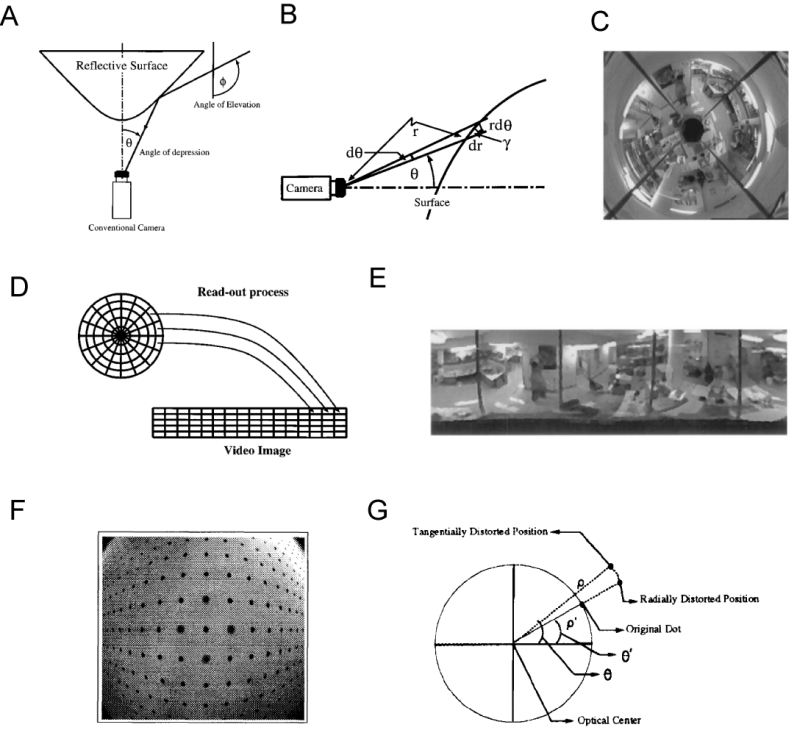
\includegraphics[width=0.75\textwidth]{vca.png}
  \caption{A) Se utiliza una cámara convencional para adquirir la imagen del espejo curvo. B) La superficie se diseña para obtener una relación lineal entre el angulo de elevacion $\phi$  y el angulo de incidencia a la camara $\theta$. C) Ejemplo de imagen adquirida por cámara. D) Algoritmo de reconstrucción de imágenes panorámicas. E) Imagen panorámica obtenida a partir de la imagen de la figura 1C.}
  \label{fig:vca}
\end{figure}


\subsection{Clasificación BKG/FRG mediante GMM}

El objetivo principal de este trabajo es desarrollar los algoritmos iniciales de una sistema VDA con VCA. Para esto es necesario adquirir las imágenes VCA e identificar las regiones en movimiento respecto al fondo estatico. La sustraccion de fondo es un método ampliamente utilizado en imágenes de proyección plana estaticas utilizado para la detección de objetos en movimiento. La justificación de este enfoque es el de la detección de los objetos que se mueven a partir de la diferencia entre el cuadro actual y un marco de referencia, a menudo llamada la "imagen de fondo" o "modelo de fondo". Como base, la imagen de fondo debe ser una representación de la escena sin objetos en movimiento y debe mantenerse actualizada periódicamente con el fin de adaptarse a las condiciones de luminosidad diferentes. Se han propuesto varios métodos para realizar la sustracción de fondo en la literatura reciente [1].
Los sistemas de VDA  necesitan de algoritmos para detectar objetos de interés que se mueven (foreground ó FRG) respecto del fondo (background ó BKG). Estos algoritmos deben adaptarse a las variaciones de luminosidad del ambiente en distintos momentos del día y también deben poder distinguir por ejemplo, entre el movimiento de ramas de árboles (que corresponden al BKG)  respecto de vehículos o personas (que corresponden al FRG). 
Existen varios métodos para realizar la sustracción de fondo que han sido propuestos en la literatura reciente. Para segmentar los objetos del FRG se desarrollaron algoritmos heurísticos (Collins et al. 2001) y algoritmos estadísticos paramétricos y no paramétricos (Stauffer y Grimson 1999; McHugh et al. 2009). Todos estos métodos tratan de clasificar eficazmente el ‘fondo o BKG’ de los ‘objetos en movimiento o FRG’ que se encuentran en capas superiores (Piccardi, 2004). El modelo paramétrico más utilizado es el Gaussian Mixture Model (GMM) propuesto por Stauffer y Grimson (1999). 
Las características básicas del modelo GMM se muestran en la figura 3. Supongamos que la cámara adquiere imágenes como en la figura 3A. Nos concentramos en el valor medido para la intensidad en los pixeles 1 y 2  (indicados con círculos). El pixel 1 apunta al cielo, y esperamos que (si no hay nubes)  la distribución de intensidad sea unimodal. Por otro lado, el pixel 2 apunta a una región donde hay un árbol (con hojas y ramas) por lo que esperamos una distribución de intensidades multimodal (porque cuando hay viento el pixel sensa la rama o las hojas). Ademas el modelo supone que  los parámetros que caracterizan la distribuciones de probabilidad de intensidad pueden tener variaciones lentas a lo largo del día (por ejemplo el color e intensidad del cielo va a ir variando) (ver figura 3B). Cada nueva medición de intensidad del pixel se contrasta con la distribución de probabilidad estimada para ese pixel y se determina si el pixel debe clasificarse como BKG o FRG (mas detalles en la sección 8.1.2).  

Problema 1: Utilizar modelos estadísticos para las imágenes adquiridas y ajustarlos para poder clasificar el background (BKG) y los objetos móviles pertenecientes al foreground (FRG). Comenzaremos con imágenes en proyección plana para simplificar el problema.

Como dijimos, el modelo estadístico más utilizado para la clasificación BKG-FRG en imágenes planas es el modelo GMM (Stauffer y Grimson 1999). Este modelo propone que la distribución de probabilidad para la intensidad X de cada pixel está dada por una mezcla de K gaussianas. Cada gaussiana está representada por el índice k:

\begin{equation}
    f_{X}\left(X|\phi\right) =
    \sum\limits_{k=1}^K P\left(k\right)f_{X|k}\left(X|k,\theta_{k}\right)
\end{equation}

\begin{equation}
    f_{X|k}\left(X|k,\theta_{k}\right) =
    \frac{1}{\left(2\pi\right)^{\frac{n}{2}}|\sum_k|^{\frac{1}{2}}}
    e^{-\frac{1}{2}\left(X-\mu_k\right)^T\sum_k^{-1}\left(X-\mu_k\right)}
\end{equation}

Cada una de las distribuciones gaussianas k describe sólo un objeto que puede estar asociado al BKG o a un objeto FRG. $P(k)=\omega_k$ es la probabilidad que el pixel X pertenezca a la clase k. En los casos prácticos, el número total de clases K, asociados a un pixel se fija entre 3 y 5. Las gaussianas son multi-variable para describir componentes de color (rojo, verde y azul) de cada pixel. Los parámetros de cada clase k son la media $\mu_k$ y la covarianza $\sum_k$. Si los valores de intensidad de cada color se suponen independientes, la matriz de covarianza se simplifica a la forma diagonal. 

Estimación de los parámetros del modelo y clasificación BKG-FRG:  Dado el modelo estadístico de la ecuación X1, se utiliza el método Expectation Maximization (método EM) para inferir los parámetros del modelo y la clase más probable k para cada pixel: 

\begin{equation}
  \begin{split}
    k & = \underset{k}{\text{argmax}} P\left(k|X,\Phi\right)
  \\
      & = \underset{k}{\text{argmax}} \omega_k f_{X|k}\left(X|k,\theta_k\right)
  \end{split}
\end{equation}

Sin embargo, como este cálculo resulta computacionalmente costoso, se realiza la siguiente aproximación: Dada una medición nueva X, se calcula la distancia a la media de cada clase. Si la distancia es menor que 2.5* de una clase, se asigna ese pixel a esa clase:

\begin{equation}
  \begin{split}
    M_{k,t} & = \begin{cases}
                  1 \text{ match }
                \\
                  0 \text{ otherwise }
                \end{cases}
  \\
            & \approx P\left(k|X_t,\Phi\right)
  \end{split}
\end{equation}

Si ninguna clase cumple el criterio, se asigna la medición a los valores de clase menos probable.
Una vez que se estimó a que clase pertenece cada pixel, se estiman  los parámetros del modelo:

\begin{equation}
  \hat{\omega}_{k,t} = \left(1 - \alpha_t\right) \omega_{k,t} + \alpha_t P\left(k|X_t,\Phi\right)
\end{equation}

\begin{equation}
  \hat{\mu}_{k,t} = \left(1 - \rho_{k,t}\right) \mu_{k,t} + \rho_{k,t} X_t
\end{equation}

\begin{equation}
  \hat{\sigma}^2_{k,t} = \left(1 - \rho_{k,t}\right) \sigma^2_{k,t} + \rho_{k,t} \left(\left(X_t-\hat{\mu}_{k,t}\right)\circ\left(X_t-\hat{\mu}_{k,t}\right)\right)
\end{equation}

\begin{equation}
  \rho_{k,t} = \frac{\alpha_t P\left(k|X_t,\Phi\right)}{\hat{\omega}_{k,t}}
\end{equation}

Finalmente, se definen que clases son ‘fondo-BKG’ ó  ‘objetos en movimiento en FRG’. Para esto, se usa el siguiente método: se calcula $\omega_k/\sigma_k$ para todas las clases del pixel y se ordenan de mayor a menor. La suposición es que las clases más probables y más compactas deben componer el ‘fondo’. De este modo las primeras B distribuciones que cumplen:

\begin{equation}
  B = \underset{b}{\text{argmin}}\left(\sum\limits_{k=1}^b \omega_k>T\right)
\end{equation}

formaran el ‘fondo’. El parámetro $T$ es un umbral asignado, que se puede interpretar como la probabilidad a priori de que el pixel se ‘fondo’.
Volviendo a la figura 1C, supongamos que a tiempo $t_2$ el vehículo se desplazó y tapó el pixel 2, entonces el valor de intensidad de este pixel se alejará mucho de la distribución de intensidades observada previamente. Por lo tanto, se le asignará una nueva clase que será clasificada como FRG porque es muy poco probable $w_k \approx 0$.

\textbf{Editar para que aplique MOG2}

\subsection{Operaciones morfológicas}

\subsection{Transformación a coordenadas cartesianas}

\subsection{Trackeo Kalman en cartesianas}

\textbf{Cuando tengamos algo hecho en python de esto lo agrego}

\section{Objetivos de este trabajo}

\textbf{En base a los resultados obtenidos. Lo escribimos despues.}

\subsection{Objetivos específicos}

Los objetivos de este proyecto están asociados a mejorar dos aspectos fundamentales de la VD. El objetivo 1 consiste en desarrollar técnicas que aumenten el campo de visión (CV) manteniendo la posibilidad de analizar regiones de interés en alta resolución. Los objetivos 2 a 4 consisten en el desarrollo de algoritmos automáticos que asistan a los operadores humanos en el análisis de los videos.
\\
Sensores:
\\1- Implementación de sistemas de adquisición de imágenes tradicionales (proyección en perspectiva) y de visión de campo amplio (espejos curvos y lentes ojo de pez). 
\\Modelos estadísticos
\\2- Implementación de algoritmos para la clasificación de videos en background (BKG) y foreground (FRG). Analizar la extensión de estos algoritmos a imágenes de VCA.
\\Algoritmos de tracking
\\3- Implementación de algoritmos para el seguimiento objetos de interés.

\section{Calibración de cámara fisheye comercial}

\subsection{Cámara fisheye utilizada}

En este trabajo utilizamos la camara VIVOTEK FE8172 (ver fig. 1). Esta cámara posee un campo visual de $(360\degree x 183\degree)$ y un sensor CCD de $1920 x 1920$ pixels [manual camara].
\\\textbf{Agregar aspectos técnicos interesantes desde el punto de vista aplicado}.

\subsection{Identificación de la cámara - Calibración}

Tambien, mostramos la notación que utilizaremos en este trabajo [10]. La cámara esta posicionada en el origen $O$ y su eje óptico es el eje $Z$. Un punto en el espacio 3D es representado en coordenadas esféricas $(R,\theta,\varphi)$ donde $\theta$ de mide desde el eje óptizo $Z$ y $\varphi$ se mide desde el eje $X$ alrededor del eje óptico. De este modo, podemos escribir:

\begin{equation}
  \begin{split}
    R & = \sqrt{X^2+Y^2+Z^2}
    \\
    \theta & = a \text{cos} \left(R/z\right)
    \\
    \varphi & = a \text{tan2} \left(Y/X\right)
  \end{split}
\end{equation}

En el plano de la imagen de la cámara el punto $P$ se proyecta en el punto $p$ en coordenadas polares $(r,\varphi)$ respecto al punto principal. En las omnicámaras con simetría de revolución, $r$ es solo función de $\theta$ $(r=r(\theta))$ y las coordenadas cartesianas del punto $p$ en el plano de la imagen serán:

\begin{equation}
  \begin{split}
    u & = r \cos\left(\varphi\right)
    \\
    v & = r \sin\left(\varphi\right)
  \end{split}
\end{equation}

\begin{figure}[!h]
  \centering
  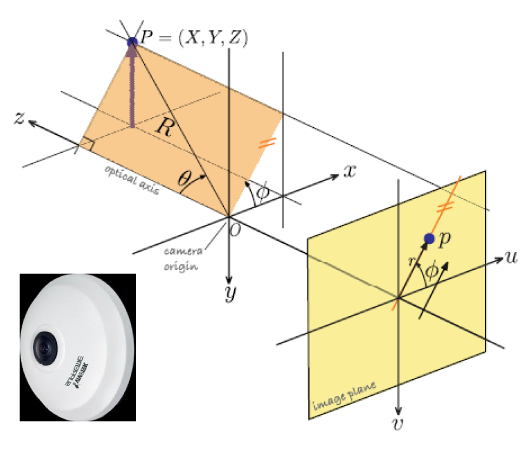
\includegraphics[width=0.6\textwidth]{coord.png}
  \caption{Camara panorámica utilizada VIVOTEK FE8172  (abajo a la izquierda) y formacion de imágenes en una cámara fisheye. El punto $P$ es representado en coordenadas esféricas $(R,\theta,\varphi)$ desde el origen de la cámara $O$ y se proyecta en el punto $p=(u,v)$ sobre la matriz CCD de la cámara. (FALTA REDIBUJAR FIGURA 1B)}
  \label{fig:coord}
\end{figure}

La distancia entre punto principal y el punto $p$, $r(\theta)$, es una función que depende del tipo de cámara fisheye que se utilice.  Existen distintos modelos de proyección que resumimos en la tabla \ref{tab:mods}.

\begin{table}[h]
  \centering
  \caption{Modelos de proyección.}
  \label{tab:mods}
  \begin{tabular}{*{2}{l}}
    \toprule
      Nombre del Modelo & Ecuación \\
    \midrule
      Estereográfico & $r(\theta) = k \tan \left(\theta/2\right)$\\
      Equiángulo & $r(\theta) = k \theta$ \\
      Equisólido & $r(\theta) = k \sin \left(\theta/2\right)$ \\
      Polinómico & $r(\theta) = k_1 \theta + k_2 \theta^2 + \dots$ \\
    \bottomrule
  \end{tabular}
\end{table}

Para calibrar la cámara fisheye utilizamos un patrón uniforme de puntos en coordenadas cartesianas. Se midieron las coordenadas esféricas $(\theta,\varphi)$ (ver figura 1B) y los datos de su proyección a través de la lente fisheye $(\theta,\varphi)$. En la figura 2B mostramos las mediciones de r vs $\theta$ y los ajustes por cuadrados minimos segun los modelos  de la tabla 1. Comparamos los ajustes de los modelos por cuadrados minimos y concluimos que el modelo que mejor ajusta la cámara VIVOTEK FE8172 es el modelo estereográfico. 

\begin{figure}[!h]
  \centering
  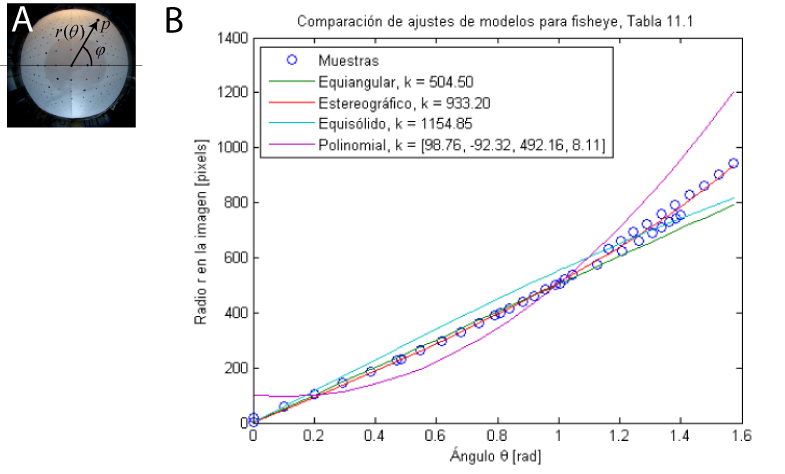
\includegraphics[width=0.75\textwidth]{ajuste.png}
  \caption{A) Patrón uniforme de puntos en coordenadas cartesianas vistos a través de la cámara fisheye. (FALTA QUE SE VEA MAS CENTRADA) B) Mediciones de $r$ vs $\theta$ y los ajustes por cuadrados minimos segun los modelos  de la tabla \ref{tab:mods}. (FALTA REVISAR AJUSTE POLINOMIO) (FALTA JUNTAR PUNTOS DOBLES)}
  \label{fig:ajuste}
\end{figure}


\subsection{Modelo unificado}

En la sección anterior hemos introducido una serie de posibles modelos para la generación de las imágenes de la  cámara y concluimos que el modelo estereográfico es el que ajusta mejor nuestra camara. Es sabido que este modelo es un caso particular de un modelo mucho más general denominado el Modelo Unificado [8]. La utilización de este modelo nos permite transformar computacionalmente una imagen capturada con una cámara central, en la imagen capturada por otra cámara central simulada. Por ejemplo, dada una proyección de una camara fisheye vamos a generar la proyección correspondiente para una cámara esférica o una cámara de perspectiva plana. Este modelo es un proceso de dos pasos y la notación se muestra en la figura 3[10].

Primero requiere la proyección esferica del punto del espacio $P = (X,Y,Z)$ en la superficie de la esfera unitaria $p' = (\theta,\varphi)$ (fig. 3, [1a]). El punto de proyección utilizado es el centro mismo de la esfera, $O = (0,0,0)$. El hecho de usar un unico punto de vista implica un sistema de vision central (fig. 3, [1b]).
El segundo paso consiste en reproyectar desde la esfera hacia el plano de la imagen ($z = -m_{fe}$). O sea, desde el punto de proyeccion $F_{fe} = (0,0,l_{fe})$ hacia el punto $p_{fe} =(r,\varphi)$ (fig. 3, [2a]). Ambos parametros, $m_{fe}$ y $l_{fe}$, dependen del tipo de camara a simular (en este caso una cámara fisheye). Según este modelo de cámara:

\begin{equation}
  r(\theta) = \frac{(l+m)\sin(\theta)}{l+\cos(\theta)}
\end{equation}

Por ejemplo, el modelo estereográfico que ajusta a la cámara VIVOTEK FE8172 equivale a un modelo unificado con ($l=1$,$m=-935$).


\section{Corrección de deformaciones locales}

\subsection{Metodo}.
Para poder transformar imágenes tomadas con la cámara VIVOTEK FE8172 en imágenes planas utilizando este modelo, también se requieren dos pasos:

- El primer consiste en proyectar desde el plano de la imagen fisheye ($z = -m_{fe} = -935$) hacia la esfera unitaria, tomando como punto de proyección $F = (0, 0, l_{fe} = 1)$.
Computacionalmente, esto se logra siguiendo estos pasos: 


\begin{enumerate}
  \item Primero se tienen las coordenadas $(u_1, v_1)$ de cada punto de la imagen fisheye, las cuales forman una malla $M_1$ (fig. 3).
  \item Se crea luego una malla $M_2$ uniforme de puntos con coordenadas ($\theta_2, \varphi_2$) que cubra el hemisferio sur de la esfera unitaria.
  \item Se proyectan estos puntos en el plano de la imagen fisheye los parámetros correspondientes al tipo de cámara con el que se tomó lo imagen, de esta manera se obtiene la malla $M_3$ con coordenadas $(u_3, v_3)$.
  \item Se interpolan las intensidades $I_1(u_1, v_1)$ de la malla $M_1$ para aproximar las intensidades $I_3(u_3, v_3)$ en la malla $M_3$.
\end{enumerate}

Este último paso se realizó con una interpolación lineal 2D, en la cual se interpolan los cuatro puntos de la malla M1 más cercanos al punto a evaluar en M3. 

Los pasos para simular una imagen tomada por una cámara plana son los siguientes:

-Proyectar nuevamente, desde la esfera unitaria hacia el plano $(z = -m_{plana})$, pero utilizando los parámetros de una imagen en perspectiva. De esta manera, el punto de proyección es $F = (0, 0, l_{plana} = 0)$. El parámetro $m_{plana}$ depende del campo de visión $\theta_{FOV}$ que se desea simular para la cámara de perspectiva y del tamaño en pixeles $W$ que se quiere tenga la imagen.

\begin{equation}
  m_{plana} = \frac{W}{2\tan\left(\frac{\theta_{FOV}}{2}\right)}
\end{equation}

La manera computacional de proceder evoca al paso 1 pero a la inversa:

\begin{enumerate}
  \item Se calcula $m_{plana}$ con la ecuación 4.
  \item Se crea la malla de puntos uniforme $(M_4)$, con coordenadas $(u_4, v_4)$ sobre el plano $(z=-m_{plana})$. 
  \item Se proyecta esta malla a la esfera unitaria utilizando los parámetros $l_{plana}=0$ y $m_{plana}$ obteniéndose la malla $M_5$ con coordenadas  $(\theta_5, \varphi_5)$.
  \item Se interpolan las intensidades $I_3(u_3, v_3)$ para obtener las intensidades $I_5(u_5, v_5)$.
\end{enumerate}

Habiendo procedido de esta manera, se obtiene la imagen en perspectiva deseada. 
 Aplicamos este esquema al patrón uniforme de la figura 4A con resultados satisfactorios. Simulamos una cámara plana con $\theta_{FOV}=150\degree$ obteniendo el patron de puntos de la figura 4B.

\begin{figure}[!h]
  \centering
  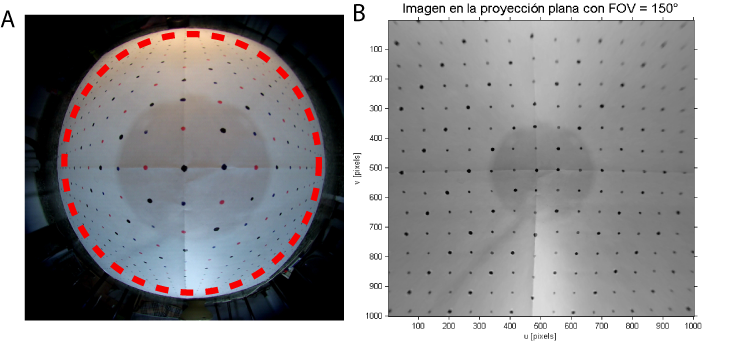
\includegraphics[width=0.75\textwidth]{afiche.png}
  \caption{Simulacion de una camara plana utilizando la imagen el patrón de calibración. A) Imagen  capturarda por la cámara fisheye. La circunferencia roja indica que se utilizará un campo de visión con $\theta_{FOV}=150\degree$. B) Simulacion de la imagen obtenida por la cámara plana utilizando el modelo unificado con $(l_{fe}=1,m_{fe}=-935)$.}
  \label{fig:afiche}
\end{figure}

\subsection{Rotación del eje principal de la cámara plana simulada}

En el ejemplo de la figura 4 el eje principal de la camara plana coincide con el de la camara fisheye. Sin embargo, podemos utilizar el modelo unificado para simular un camara PTZ plana cuyo eje principal está rotado un angulo $(\theta_{PTZ},\varphi_{PTZ})$ respecto al eje $Z$. Para simular un cámara plana rotada debemos girar la proyección esférica obtenida en el primer paso $(M_2)$ orientando su polo sur en la dirección a enfocar y luego aplicar el método anterior [11]. Suponiendo que el operador indica que la región de interés está centrada en el pixel (uptz, vptz), los pasos para orientar la la malla $M_2$ en esa dirección son los siguientes:

\begin{enumerate}
  \item Invirtiendo la ec. 2, se calculan las coordenadas $(\theta_{PTZ},\varphi_{PTZ})$ correspondientes al punto $(u_{PTZ},v_{PTZ})$ y se crea un versor  asociado a  $(\theta_{PTZ},\varphi_{PTZ},1)$ que indica hacia donde se quiere apuntar la cámara PTZ simulada.
  \item Se calcula el versor sobre el cual se girará la malla $M_2$ sobre la esfera como el producto cruz.
  \item Una vez conocido el eje de giro , se calcula la matriz de rotación $R_k(-\theta)$ y se aplica esta transformación a todos los puntos de la malla $M_2$.
\end{enumerate}

Luego de estos pasos se aplica el método desarrollado para el caso de ejes paralelos en las dos cámaras 

\pagebreak

\section{Detección de objetos múltiples}
\subsection{Clasificación BKG/FRG mediante MOG2}

El método general más común para detectar regiones en movimiento en un video en tiempo real comprende la llamada sustracción de fondo. Ésta consiste básicamente en comparar la imagen actual contra una estimación de la imagen sin objetos en movimiento. Si el error es mayor a cierto umbral, se considera que esa región, efectivamente, no pertenece al fondo.

Los numerosos acercamientos a este problema difieren entre sí en dos aspectos principales: el tipo de modelo de fondo (background - BKG) y el procedimiento usado para actualizar el mismo.

Debido a su eficiencia y poco requerimiento computacional, actualmente los métodos más populares comprenden el modelado mediante mezclas de gaussianas. 
Esto quiere decir que cada pixel de la estimación del fondo es representado como una distribución de probabilidad resultado de combinar de distribuciones gaussianas






Para la detección de objetos en el video obtenido por la cámara, se aprovecharon las librerías open source de OpenCV. Del grupo de algoritmos disponibles se eligió aquel llamado MOG2 \cite{zivkovic2004} \cite{zivkovic2006} que además de detectar objetos en movimiento, permite identificar las sombras.
\\
Básicamente, este algoritmo pretende obtener un modelo del fondo (background - BKG) y, al obtener un fotograma en el tiempo $t$ comparar cada pixel $X_t$ con el modelo para determinar si pertenece al BKG o a un objeto en movimiento (foreground - FRG).
En este algoritmo en particular, el modelo de cada pixel se da como una mezcla de distribuciones Gaussianas referidas al vector de color, donde cada uno de los parámetros que definen a esas distribuciones se actualiza mediante la siguiente regla \cite{titterington1984}:

!!!! Meter todo esto en una fórmula con split

\begin{equation}
  \omega_{k,t} \leftarrow \omega_{k,t} + \alpha \left( M_{k,t} - \omega_{k,t}\right)
\end{equation}
\begin{equation}
  \delta_{k,t} \leftarrow X_t - \mu_{k,t}
\end{equation}
\begin{equation}
  \mu_{k,t} \leftarrow \mu_{k,t} + M_{k,t} \left( \alpha / \omega_{k,t} \right) \delta_{k,t}
\end{equation}
\begin{equation}
  \sigma^2_{k,t} \leftarrow \sigma^2_{k,t} + \mu_{k,t} + M_{k,t} \left( \alpha / \omega_{k,t} \right) \left( \delta^T_{k,t} \delta_{k,t} - \sigma^2_{k,t}\right)
\end{equation}

!!!!Explicar los parámetros customizables del algoritmo primero, utilizando datos del paper, y luego mencionar los ajustes elegidos

\begin{equation}
  B = \underset{b}{\text{argmin}}\left(\sum\limits^b_{k=1}\omega_k>(1-c_f)\right)
\end{equation}

!!!!En las ecuaciones de Stauffer & Grimson se usa como umbral para la sumatoria anterior $T$, pero no la $T$ de cantidad de frames que usamos acá.
¿Cuál de los dos usamos: $(1-c_f)$ ó $T$? Mi apuesta iría por un tercero: $\Omega$ o $C$.

!!!!Cómo reconciliar el GMM de la introducción con el que usamos en realidad. Cuánto desarrollar en la introducción y qué dar por sentado acá.

\subsection{Máscara ROI}

!!!!Sería genial lograr una GUI para hacer más amigable la definición de máscaras. Estuve investigando de esto, PyGTK parece hacer el trabajo. Igual es un endgame topic.

\subsection{Cálculo de posición y tamaño del objeto en cartesianas}


\pagebreak

!!!!Sigo rompiéndome la cabeza viendo cómo citar correctamente con Bibtex.

\bibliography{st15}{}
\bibliographystyle{plain}

\end{document}
